\chapter{Sistema Linfatico}

\section{Cenni di Anatomia e Fisiologia}
Il sistema linfatico \`e una componente essenziale del sistema immunitario, 
insieme a milza, midollo osseo, timo, tonsille, appendice ciecale e placche di Peyer. 
Esso si compone di organi linfatici e vasi linfatici e rappresenta 
un sistema di drenaggio parallelo a quello venoso\cite{BOOK1}, come in Figura \ref{fig:FIGURE_1.1}.\\

\begin{figure}[H]
    \begin{center}
    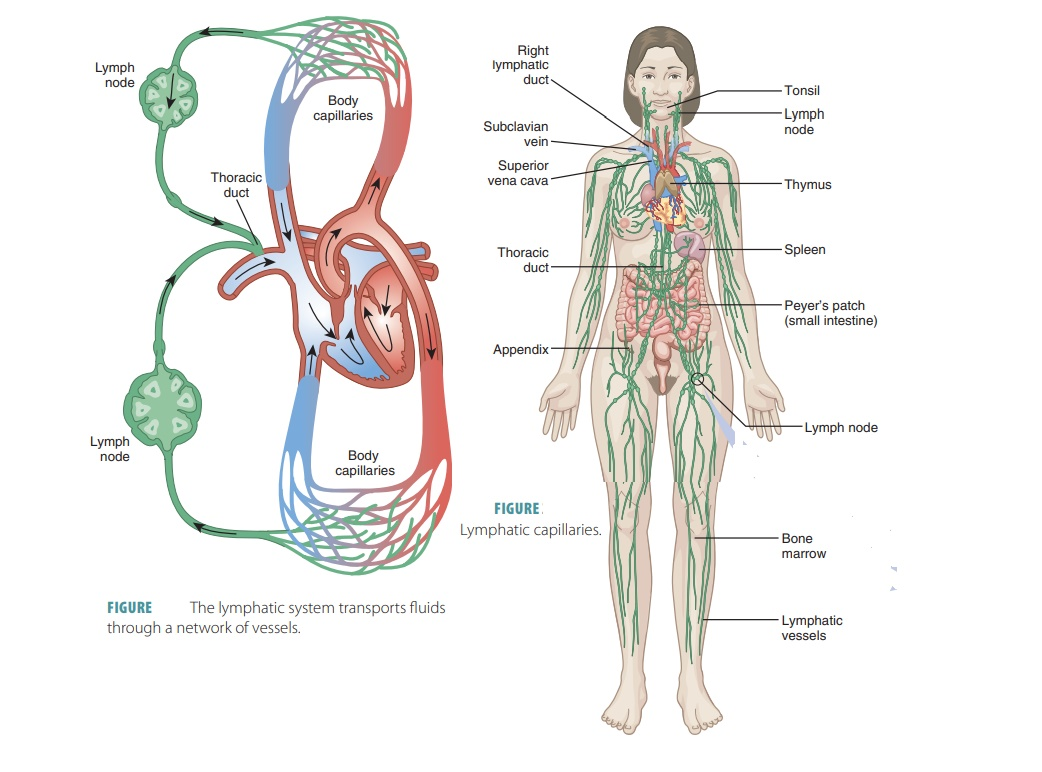
\includegraphics[width=0.9\columnwidth]{img/ANATOMY2.jpeg}
    \end{center}
    \caption{Anatomia del sistema linfatico, circolazione sanguignia e linfatica
    \cite{img1}}
    \label{fig:FIGURE_1.1}
\end{figure}


Gli organi linfatici sono suddivisi in primari o centrali 
e secondari o periferici; gli organi linfatici primari sono midollo osseo 
e timo, al loro interno i linfociti maturano per diventare linfociti T (nel timo) 
o linfociti B (nel midollo osseo). 
Gli organi linfatici secondari sono linfonodi, milza, e MALT 
(tessuto linfoide associato alle mucose) costituito da tonsille, 
placche di Peyer, appendice ciecale e altri raggruppamenti linfocitari 
sparsi nelle mucose (Figura \ref{fig:FIGURE_1.2}). Gli organi linfoidi secondari, hanno un ruolo fondamentale 
nella risposta immunitaria, in quanto, i linfociti attivati, svolgono le loro funzioni 
in seguito al contatto con l'antigene\cite{BOOK1}.\\

\begin{figure}[H]
    \begin{center}
    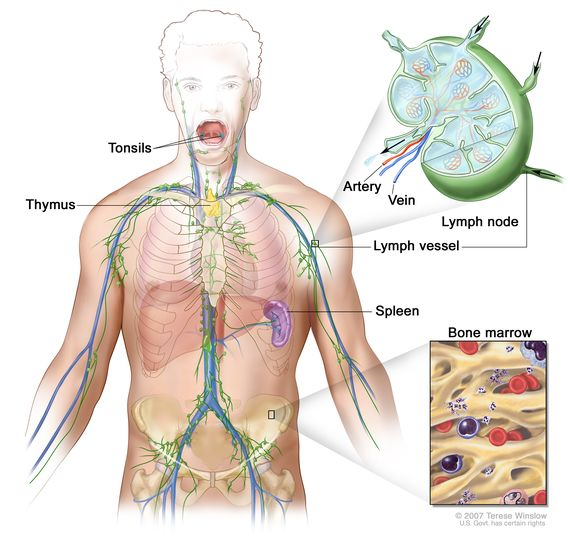
\includegraphics[width=0.5\columnwidth]{img/anatomy.jpeg}
    \end{center}
    \caption{Organi linfatici, struttura di linfonodi e midollo osseo
    \cite{img2}}
    \label{fig:FIGURE_1.2}
\end{figure}

I vasi linfatici possiedono strutture valvolari che garantiscono un flusso monodirezionale; 
il sistema linfatico infatti non possiede una pompa centrale, 
come avviene per il sistema circolatorio, ma la linfa scorre grazie ad una motricit\'a spontanea delle pareti.\\
Il sistema linfatico presenta delle interruzioni lungo il suo decorso: i linfonodi. 
I linfonodi filtrano e depurano la linfa dai microrganismi, dalle cellule neoplastiche e 
da particelle estranee. Essi si raggruppano nelle aree da cui si diramano i vasi linfatici, 
come collo, ascelle e inguine.\\
La linfa \'e il tessuto connettivo fluido trasportato e regolato da tale sistema, \'e costituita 
da liquidi che trasudano nei tessuti dell'organismo, tramite le pareti dei capillari; essa \'e costituita 
da ossigeno, proteine, globuli bianchi e altre sostanze nutrienti.\\ 
La linfa trasporta sostanze estranee (batteri), cellule tumorali, cellule morte o danneggiate.\\ 
I vasi linfatici pi\'u piccoli si collegano a quelli pi\'u grandi e formano il dotto linfatico e il dotto 
toracico, quest'ultimo \'e il vaso linfatico pi\'u grande, che si collega alla vena succlavia per poi restituire 
la linfa alla circolazione sanguigna\cite{BOOK1}. \\

\section{Funzioni del Sistema Linfatico}
Le funzioni del sistema linfatico sono la produzione, il mantenimento e la distribuzione dei linfociti, 
il mantenimento della volemia ed anche la via alternativa per il trasporto di ormoni,
sostanze nutritizie e di scarto\cite{BOOK1}.\\
I linfociti sono indispensabili per i normali meccanismi di difesa, vengono prodotti e accumulati a livello 
degli organi linfoidi. 
A livello degli organi linfoidi primari, midollo osseo e timo, si ha lo sviluppo e la maturazione dei linfociti 
i quali successivamente si differenzieranno in cellule B, T o NK (natural killer)\cite{BOOK1}.
La risposta immunitaria inizia a livello degli organi linfoidi secondari: la polpa bianca della milza, le tonsille, 
l’appendice, le placche di peyer e i linfonodi, dove in caso di infezione, ad esempio,
i linfociti B si dividono per produrre ulteriori linfociti B, necessari a debellare l’infezione.\\
Il sistema linfatico, ha un ruolo importante nel mantenimento della volemia (volume sanguigno) in quanto 
quotidianamente si ha un movimento di un notevole quantitativo di liquidi attraverso il sistema linfatico e 
la rottura di uno dei vasi linfatici può portare ad una rapida,nonché fatale, diminuzione della volemia\cite{BOOK1}.\\
Esso rappresenta inoltre una via alternativa per il trasporto di ormoni, sostanze nutritizie e 
di scarto in quanto alcune sostanze, come anche alcuni lipidi, vengono assorbiti nel circolo sanguigno tramite 
i vasi linfatici, piuttosto che per assorbimento da parte delle pareti dei capillari\cite{BOOK1}.\\

\section{I vasi linfatici}
La linfa che scorre nei capillari linfatici, viene raccolta da due gruppi di vasi linfatici: i vasi linfatici 
superficiali e i vasi linfatici profondi.\\ 
I vasi linfatici superficiali si trovano nel tessuto sottocutaneo, nei tessuti connettivi lassi delle membrane sierose 
(cavità pleurica, pericardica e peritoneale) e mucose (apparati digerente, respiratorio, urinario e riproduttivo).\\ 
I vasi linfatici profondi raccolgono la linfa proveniente dalla muscolatura scheletrica, da collo, arti, tronco, 
dai visceri delle cavità toracica e addominopelvica\cite{BOOK1}.\\
Nel tronco, i vasi linfatici superficiali e profondi convergono a formare vasi di calibro maggiore, 
i tronchi linfatici (includono i tronchi lombari, intestinali, broncomediastinici, succlavii, giugulari), 
che a loro volta si svuotano in due grossi vasi collettori, i dotti linfatici, che convogliano la linfa 
nella circolazione venosa.\\  
Il dotto toracico, che è il vaso linfatico più grande, raccoglie la linfa da tutta la porzione sottodiaframmatica 
del corpo e dalla metà sinistra sopradiaframmatica; si svuota nel punto di confluenza della vena succlavia sinistra e 
in tal modo, nel sistema venoso, rientra la linfa proveniente dal lato sinistro di testa, collo, torace e 
dall’intera porzione sottodiaframmatica del corpo.\\ 
Il dotto linfatico destro ha un diametro relativamente ridotto e raccoglie la linfa dalla metà destra 
del corpo superiore al diaframma. Essa si svuota nel punto in cui confluiscono la vena giugulare interna destra e la 
vena succlavia destra\cite{BOOK1}.\\
 

\section{Linfociti}
I linfociti rappresentano il tipo cellulare principale del sistema linfatico. 
Essi sono deputati all'immunità specifica e intervengono per eliminare agenti estranei 
(virus, batteri, cellule neoplastiche, tossine batteriche) o per renderli inoffensivi. 
I principali tipi di linfociti sono le cellule T (timo dipendenti) e le cellule B (bone marrow-derived)\cite{BOOK2}.\\
I linfociti T rappresentano circa l’80\% dei linfociti circolanti, essi originano dal midollo osseo, 
poi migrano nel timo dove si differenziano e diventano immunocompetenti. 
Vi sono due sottoclassi di linfociti T: i linfociti T-helper e i linfociti T citotossici o NK (natural killer). 
I linfociti NK rappresentano il 5-10\% dei linfociti circolanti e insieme ai macrofagi attivati, 
sono responsabili della sorveglianza immunitaria grazie al controllo costante dei tessuti periferici.\\
I linfociti B rappresentano il 10-15\% dei linfociti circolanti, originano e diventano immunocompetenti 
nel midollo osseo e la loro funzione principale è quella di trasformarsi in plasmacellule, 
per produrre e secernere anticorpi\cite{BOOK2}.\\   

\section{Patologie del sistema linfatico: i linfomi}
I linfomi, sono tumori maligni, che originano dalla proliferazione incontrollata dei linfociti o di cellule staminali 
linfoidi. Tale proliferazione incontrollata, è causata dalla comparsa di mutazioni dei geni coinvolti 
nella maturazione, nella crescita e nella morte dei linfociti, 
che possono infatti acquisire la capacità di replicarsi in modo incontrollato\cite{LINFOMIAIL}.\\ 
I linfomi presentano caratteristiche estremamente variabili, proprio in virtù delle molteplici mutazioni 
che possono insorgere nelle diverse fasi dello sviluppo del linfocita. 
I linfociti si accumulano e invadono più frequentemente i linfonodi, ma possono localizzarsi anche in altri organi.\\
I fattori scatenanti tale malattia sono in gran parte sconosciuti, tuttavia alcune infezioni da parte di virus e 
batteri, nonché alcune malattie croniche, aumentano il rischio di sviluppare alcuni sottotipi di linfoma\cite{LINFOMIAIL}.\\

I linfomi sono suddivisi in Linfomi di Hodgkin e Linfomi non-Hodgkin; 
i primi sono dovuti alla trasformazione dei linfociti B, i secondi possono coinvolgere sia linfociti B che T.\\ 
La modalità di crescita e progressione della malattia è un aspetto importante per la classificazione dei linfomi.
La strategia terapeutica da attuare e la prognosi dipendono dal tipo di malattia e dalla sua velocità di 
progressione\cite{LINFOMIAIL}.\\





